\subsubsection{Wards}

\begin{center}
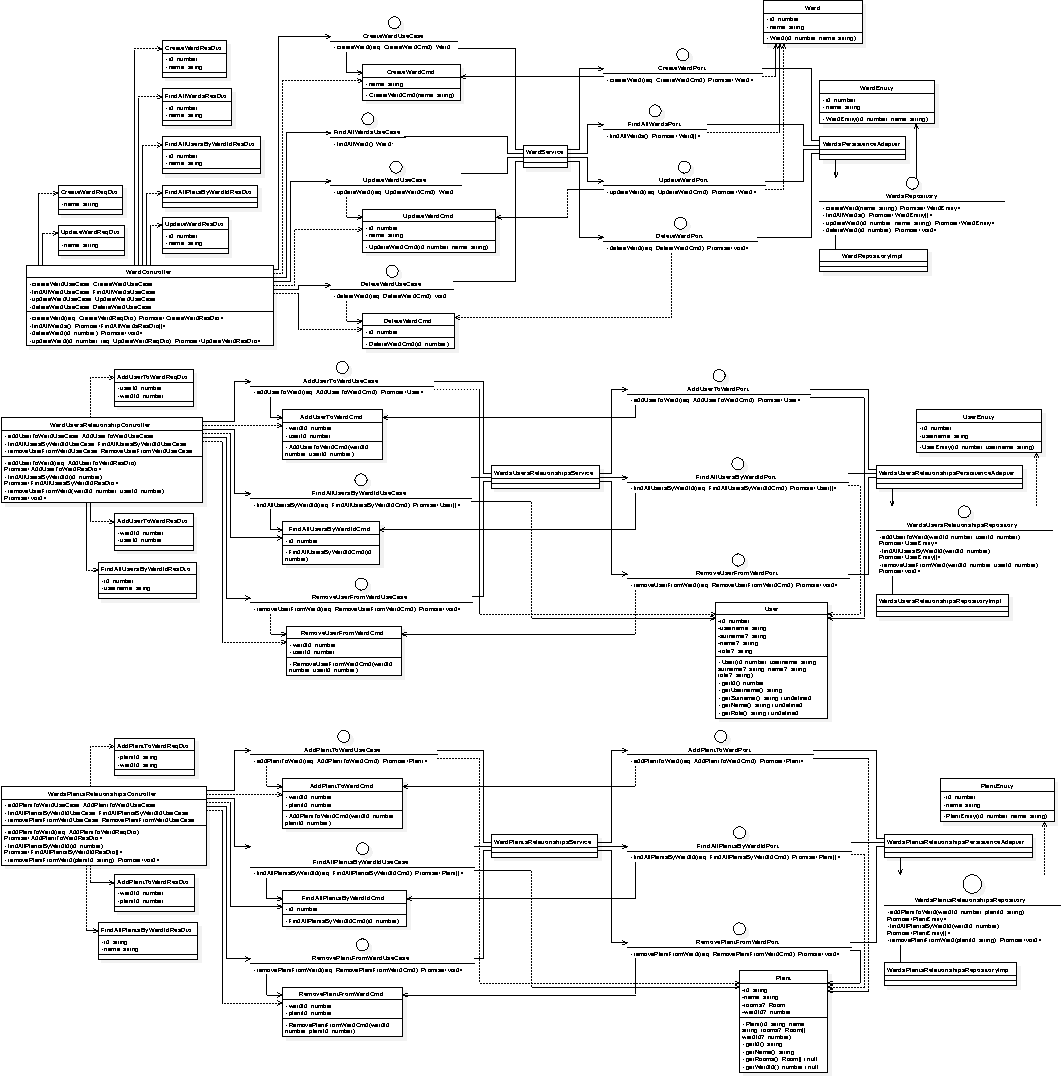
\includegraphics[width=\textwidth]{./backend/wards/wards.pdf}
\captionof{figure}{Diagramma delle classi del modulo Wards}
\end{center}

% req in

\addAtr{}{plantId: string}{Identificativo dell'impianto da associare al ward}
\addAtr{}{wardId: number}{Identificativo del ward a cui aggiungere l'impianto}
\makeCl{AddPlantToWardReqDto}{DTO di richiesta per l'associazione di un impianto a un ward}

\addAtr{}{userId: number}{Identificativo dell'utente da associare al ward}
\addAtr{}{wardId: number}{Identificativo del ward a cui aggiungere l'utente}
\makeCl{AddUserToWardReqDto}{DTO di richiesta per l'associazione di un utente a un ward}

\addAtr{}{name: string}{Nome da assegnare al nuovo ward}
\makeCl{CreateWardReqDto}{DTO di richiesta per la creazione di un nuovo ward}

\addAtr{}{name: string}{Nuovo nome da assegnare al ward}
\makeCl{UpdateWardReqDto}{DTO di richiesta per l'aggiornamento del nome di un ward}

% req out

\addAtr{}{id: string}{Identificativo univoco dell'impianto associato}
\addAtr{}{name: string}{Nome dell'impianto associato al ward}
\makeCl{AddPlantToWardResDto}{DTO di risposta restituito dopo l'associazione di un impianto a un ward}

\addAtr{}{id: number}{Identificativo univoco dell'utente associato}
\addAtr{}{name: string}{Nome dell'utente associato al ward}
\makeCl{AddUserToWardResDto}{DTO di risposta restituito dopo l'associazione di un utente a un ward}

\addAtr{}{id: number}{Identificativo univoco del ward creato}
\addAtr{}{name: string}{Nome del ward creato}
\makeCl{CreateWardResDto}{DTO di risposta restituito dopo la creazione di un nuovo ward}

\addAtr{}{id: string}{Identificativo univoco dell'impianto}
\addAtr{}{name: string}{Nome dell'impianto}
\makeCl{FindAllPlantsByWardIdResDto}{DTO di risposta per un elemento della lista degli impianti associati a un ward}

\addAtr{}{id: number}{Identificativo univoco dell'utente}
\addAtr{}{username: string}{Username dell'utente associato al ward}
\makeCl{FindAllUsersByWardIdResDto}{DTO di risposta per un elemento della lista degli utenti associati a un ward}

\addAtr{}{id: number}{Identificativo univoco del ward}
\addAtr{}{name: string}{Nome del ward}
\makeCl{FindAllWardsResDto}{DTO di risposta per un elemento della lista di tutti i ward del sistema}

\addAtr{}{id: number}{Identificativo univoco del ward aggiornato}
\addAtr{}{name: string}{Nome aggiornato del ward}
\makeCl{UpdateWardResDto}{DTO di risposta restituito dopo l'aggiornamento di un ward}

% model

\addAtr{+}{id: number}{Identificativo univoco dell'utente}
\addAtr{+}{username: string}{Username dell'utente}
\makeCl{User}{Modello di dominio che rappresenta un utente nel contesto del modulo Wards}

\addAtr{+}{id: number}{Identificativo univoco del ward}
\addAtr{+}{name: string}{Nome del ward}
\makeCl{Ward}{Modello di dominio che rappresenta un ward del sistema}

% controller

\addAtr{-}{addPlantToWardUseCase: AddPlantToWardUseCase}{Use case per l'associazione di un impianto a un ward}
\addAtr{-}{findAllPlantsByWardIdUseCase: FindAllPlantsByWardIdUseCase}{Use case per il recupero degli impianti associati a un ward}
\addAtr{-}{removePlantFromWardUseCase: RemovePlantFromWardUseCase}{Use case per la rimozione di un impianto da un ward}
\addMet{+}{addPlantToWard(req: AddPlantToWardReqDto): Promise$<$AddPlantToWardResDto$>$}{Espone l'endpoint per l'associazione di un impianto a un ward}
\addMet{+}{findAllPlantsByWardId(id: number): Promise$<$FindAllPlantsByWardIdResDto[]$>$}{Espone l'endpoint per il recupero di tutti gli impianti associati a un ward}
\addMet{+}{removePlantFromWard(plantId: string): Promise$<$void$>$}{Espone l'endpoint per la rimozione di un impianto da un ward}
\makeCl{WardsPlantsRelationshipsController}{Controller REST che gestisce le richieste HTTP relative alle associazioni tra ward e impianti}

\addAtr{-}{addUserToWardUseCase: AddUserToWardUseCase}{Use case per l'associazione di un utente a un ward}
\addAtr{-}{findAllUsersByWardIdUseCase: FindAllUsersByWardIdUseCase}{Use case per il recupero degli utenti associati a un ward}
\addAtr{-}{removeUserFromWardUseCase: RemoveUserFromWardUseCase}{Use case per la rimozione di un utente da un ward}
\addMet{+}{addUserToWard(req: AddUserToWardReqDto): Promise$<$AddUserToWardResDto$>$}{Espone l'endpoint per l'associazione di un utente a un ward}
\addMet{+}{findAllUsersByWardId(id: number): Promise$<$FindAllUsersByWardIdResDto[]$>$}{Espone l'endpoint per il recupero di tutti gli utenti associati a un ward}
\addMet{+}{removeUserFromWard(wardId: number, userId: number): Promise$<$void$>$}{Espone l'endpoint per la rimozione di un utente da un ward}
\makeCl{WardsUsersRelationshipsController}{Controller REST che gestisce le richieste HTTP relative alle associazioni tra ward e utenti}

\addAtr{-}{createWardUseCase: CreateWardUseCase}{Use case per la creazione di un nuovo ward}
\addAtr{-}{findAllWardUseCase: FindAllWardsUseCase}{Use case per il recupero di tutti i ward}
\addAtr{-}{updateWardUseCase: UpdateWardUseCase}{Use case per l'aggiornamento di un ward}
\addAtr{-}{deleteWardUseCase: DeleteWardUseCase}{Use case per l'eliminazione di un ward}
\addMet{+}{createWard(req: CreateWardReqDto): Promise$<$CreateWardResDto$>$}{Espone l'endpoint per la creazione di un nuovo ward}
\addMet{+}{findAllWards(): Promise$<$FindAllWardsResDto[]$>$}{Espone l'endpoint per il recupero di tutti i ward del sistema}
\addMet{+}{updateWard(id: number, req: UpdateWardReqDto): Promise$<$UpdateWardResDto$>$}{Espone l'endpoint per l'aggiornamento del nome di un ward}
\addMet{+}{deleteWard(id: number): Promise$<$void$>$}{Espone l'endpoint per l'eliminazione di un ward}
\makeCl{WardsController}{Controller REST che gestisce le richieste HTTP relative alle operazioni CRUD sui ward}

% command

\addAtr{+}{wardId: number}{Identificativo del ward a cui aggiungere l'impianto}
\addAtr{+}{plantId: string}{Identificativo dell'impianto da associare}
\makeCl{AddPlantToWardCmd}{Comando per l'associazione di un impianto a un ward}

\addAtr{+}{wardId: number}{Identificativo del ward a cui aggiungere l'utente}
\addAtr{+}{userId: number}{Identificativo dell'utente da associare}
\makeCl{AddUserToWardCmd}{Comando per l'associazione di un utente a un ward}

\addAtr{+}{name: string}{Nome da assegnare al nuovo ward}
\makeCl{CreateWardCmd}{Comando per la creazione di un nuovo ward}

\addAtr{+}{id: number}{Identificativo del ward da eliminare}
\makeCl{DeleteWardCmd}{Comando per l'eliminazione di un ward}

\addAtr{+}{id: number}{Identificativo del ward di cui recuperare gli impianti}
\makeCl{FindAllPlantsByWardIdCmd}{Comando per il recupero di tutti gli impianti associati a un ward}

\addAtr{+}{id: number}{Identificativo del ward di cui recuperare gli utenti}
\makeCl{FindAllUsersByWardIdCmd}{Comando per il recupero di tutti gli utenti associati a un ward}

\addAtr{+}{plantId: string}{Identificativo dell'impianto da rimuovere dal ward}
\makeCl{RemovePlantFromWardCmd}{Comando per la rimozione di un impianto da un ward}

\addAtr{+}{wardId: number}{Identificativo del ward da cui rimuovere l'utente}
\addAtr{+}{userId: number}{Identificativo dell'utente da rimuovere}
\makeCl{RemoveUserFromWardCmd}{Comando per la rimozione di un utente da un ward}

\addAtr{+}{id: number}{Identificativo del ward da aggiornare}
\addAtr{+}{name: string}{Nuovo nome da assegnare al ward}
\makeCl{UpdateWardCmd}{Comando per l'aggiornamento del nome di un ward}

% use case

\addMet{+}{addPlantToWard(req: AddPlantToWardCmd): Promise$<$Plant$>$}{Associa un impianto al ward specificato e restituisce il modello dell'impianto aggiunto}
\makeItf{AddPlantToWardUseCase}{Interfaccia del use case per l'associazione di un impianto a un ward}

\addMet{+}{addUserToWard(req: AddUserToWardCmd): Promise$<$User$>$}{Associa un utente al ward specificato e restituisce il modello dell'utente aggiunto}
\makeItf{AddUserToWardUseCase}{Interfaccia del use case per l'associazione di un utente a un ward}

\addMet{+}{createWard(req: CreateWardCmd): Promise$<$Ward$>$}{Crea un nuovo ward e restituisce il modello creato}
\makeItf{CreateWardUseCase}{Interfaccia del use case per la creazione di un nuovo ward}

\addMet{+}{deleteWard(req: DeleteWardCmd): Promise$<$void$>$}{Elimina il ward identificato dal comando}
\makeItf{DeleteWardUseCase}{Interfaccia del use case per l'eliminazione di un ward}

\addMet{+}{findAllPlantsByWardId(req: FindAllPlantsByWardIdCmd): Promise$<$Plant[]$>$}{Recupera tutti gli impianti associati al ward specificato}
\makeItf{FindAllPlantsByWardIdUseCase}{Interfaccia del use case per il recupero degli impianti di un ward}

\addMet{+}{findAllUsersByWardId(req: FindAllUsersByWardIdCmd): Promise$<$User[]$>$}{Recupera tutti gli utenti associati al ward specificato}
\makeItf{FindAllUsersByWardIdUseCase}{Interfaccia del use case per il recupero degli utenti di un ward}

\addMet{+}{findAllWards(): Promise$<$Ward[]$>$}{Recupera tutti i ward configurati nel sistema}
\makeItf{FindAllWardsUseCase}{Interfaccia del use case per il recupero di tutti i ward}

\addMet{+}{removePlantFromWard(req: RemovePlantFromWardCmd): Promise$<$void$>$}{Rimuove l'associazione tra un impianto e il ward a cui appartiene}
\makeItf{RemovePlantFromWardUseCase}{Interfaccia del use case per la rimozione di un impianto da un ward}

\addMet{+}{removeUserFromWard(req: RemoveUserFromWardCmd): Promise$<$void$>$}{Rimuove l'associazione tra un utente e il ward a cui è assegnato}
\makeItf{RemoveUserFromWardUseCase}{Interfaccia del use case per la rimozione di un utente da un ward}

\addMet{+}{updateWard(req: UpdateWardCmd): Promise$<$Ward$>$}{Aggiorna il nome del ward e restituisce il modello aggiornato}
\makeItf{UpdateWardUseCase}{Interfaccia del use case per l'aggiornamento di un ward}

% service

\addAtr{-}{findAllWardsPort: FindAllWardsPort}{Porta per il recupero di tutti i ward}
\addMet{+}{createWard(req: CreateWardCmd): Promise$<$Ward$>$}{Crea un nuovo ward delegando alla porta di persistenza}
\addMet{+}{findAllWards(): Promise$<$Ward[]$>$}{Recupera tutti i ward delegando alla porta di persistenza}
\addMet{+}{updateWard(req: UpdateWardCmd): Promise$<$Ward$>$}{Aggiorna un ward delegando alla porta di persistenza}
\addMet{+}{deleteWard(req: DeleteWardCmd): Promise$<$void$>$}{Elimina un ward delegando alla porta di persistenza}
\makeCl{WardService}{Servizio applicativo che implementa i use case relativi alle operazioni CRUD sui ward}

\addAtr{-}{addPlantToWardPort: AddPlantToWardPort}{Porta per l'associazione di un impianto a un ward}
\addAtr{-}{findAllPlantsByWardIdPort: FindAllPlantsByWardIdPort}{Porta per il recupero degli impianti di un ward}
\addAtr{-}{removePlantFromWardPort: RemovePlantFromWardPort}{Porta per la rimozione di un impianto da un ward}
\addMet{+}{addPlantToWard(req: AddPlantToWardCmd): Promise$<$Plant$>$}{Associa un impianto a un ward delegando alla porta di persistenza}
\addMet{+}{findAllPlantsByWardId(req: FindAllPlantsByWardIdCmd): Promise$<$Plant[]$>$}{Recupera gli impianti di un ward delegando alla porta di persistenza}
\addMet{+}{removePlantFromWard(req: RemovePlantFromWardCmd): Promise$<$void$>$}{Rimuove un impianto da un ward delegando alla porta di persistenza}
\makeCl{WardsPlantsRelationshipsService}{Servizio applicativo che implementa i use case relativi alle associazioni tra ward e impianti}

\addAtr{-}{addUserToWardPort: AddUserToWardPort}{Porta per l'associazione di un utente a un ward}
\addAtr{-}{findAllUsersByWardIdPort: FindAllUsersByWardIdPort}{Porta per il recupero degli utenti di un ward}
\addAtr{-}{removeUserFromWardPort: RemoveUserFromWardPort}{Porta per la rimozione di un utente da un ward}
\addMet{+}{addUserToWard(req: AddUserToWardCmd): Promise$<$User$>$}{Associa un utente a un ward delegando alla porta di persistenza}
\addMet{+}{findAllUsersByWardId(req: FindAllUsersByWardIdCmd): Promise$<$User[]$>$}{Recupera gli utenti di un ward delegando alla porta di persistenza}
\addMet{+}{removeUserFromWard(req: RemoveUserFromWardCmd): Promise$<$void$>$}{Rimuove un utente da un ward delegando alla porta di persistenza}
\makeCl{WardsUsersRelationshipsService}{Servizio applicativo che implementa i use case relativi alle associazioni tra ward e utenti}

% port

\addMet{+}{addPlantToWard(req: AddPlantToWardCmd): Promise$<$Plant$>$}{Persiste l'associazione tra un impianto e un ward e restituisce il modello dell'impianto}
\makeItf{AddPlantToWardPort}{Porta di uscita per l'associazione di un impianto a un ward}

\addMet{+}{addUserToWard(req: AddUserToWardCmd): Promise$<$User$>$}{Persiste l'associazione tra un utente e un ward e restituisce il modello dell'utente}
\makeItf{AddUserToWardPort}{Porta di uscita per l'associazione di un utente a un ward}

\addMet{+}{createWard(req: CreateWardCmd): Promise$<$Ward$>$}{Persiste il nuovo ward e restituisce il modello creato}
\makeItf{CreateWardPort}{Porta di uscita per la creazione e persistenza di un nuovo ward}

\addMet{+}{deleteWard(req: DeleteWardCmd): Promise$<$void$>$}{Elimina il ward specificato dal livello di persistenza}
\makeItf{DeleteWardPort}{Porta di uscita per l'eliminazione di un ward}

\addMet{+}{findAllPlantsByWardId(req: FindAllPlantsByWardIdCmd): Promise$<$Plant[]$>$}{Recupera dal livello di persistenza tutti gli impianti associati al ward specificato}
\makeItf{FindAllPlantsByWardIdPort}{Porta di uscita per il recupero degli impianti di un ward}

\addMet{+}{findAllUsersByWardId(req: FindAllUsersByWardIdCmd): Promise$<$User[]$>$}{Recupera dal livello di persistenza tutti gli utenti associati al ward specificato}
\makeItf{FindAllUsersByWardIdPort}{Porta di uscita per il recupero degli utenti di un ward}

\addMet{+}{findAllWards(): Promise$<$Ward[]$>$}{Recupera dal livello di persistenza tutti i ward del sistema}
\makeItf{FindAllWardsPort}{Porta di uscita per il recupero di tutti i ward}

\addMet{+}{removePlantFromWard(req: RemovePlantFromWardCmd): Promise$<$void$>$}{Elimina dal livello di persistenza l'associazione tra l'impianto e il suo ward}
\makeItf{RemovePlantFromWardPort}{Porta di uscita per la rimozione di un impianto da un ward}

\addMet{+}{removeUserFromWard(req: RemoveUserFromWardCmd): Promise$<$void$>$}{Elimina dal livello di persistenza l'associazione tra l'utente e il ward}
\makeItf{RemoveUserFromWardPort}{Porta di uscita per la rimozione di un utente da un ward}

\addMet{+}{updateWard(req: UpdateWardCmd): Promise$<$Ward$>$}{Aggiorna il ward nel livello di persistenza e restituisce il modello aggiornato}
\makeItf{UpdateWardPort}{Porta di uscita per l'aggiornamento di un ward}

% entity

\addAtr{+}{id: string}{Identificativo univoco dell'impianto nel database}
\addAtr{+}{name: string}{Nome dell'impianto}
\makeCl{PlantEntity}{Entità di persistenza che rappresenta un impianto nel contesto del modulo Wards}

\addAtr{+}{id: number}{Identificativo univoco dell'utente nel database}
\addAtr{+}{username: string}{Username dell'utente}
\makeCl{UserEntity}{Entità di persistenza che rappresenta un utente nel contesto del modulo Wards}

\addAtr{+}{id: number}{Identificativo univoco del ward nel database}
\addAtr{+}{name: string}{Nome del ward}
\makeCl{WardEntity}{Entità di persistenza che rappresenta un ward nel database}

% adapter

\addAtr{-}{wardsRepository: WardsRepository}{Repository per l'accesso ai dati dei ward nel database}
\addMet{+}{createWard(req: CreateWardCmd): Promise$<$Ward$>$}{Delega al repository la creazione del ward e mappa il risultato nel modello di dominio}
\addMet{+}{findAllWards(): Promise$<$Ward[]$>$}{Recupera e mappa tutti i ward dal repository}
\addMet{+}{updateWard(req: UpdateWardCmd): Promise$<$Ward$>$}{Delega al repository l'aggiornamento del ward e mappa il risultato nel modello di dominio}
\addMet{+}{deleteWard(req: DeleteWardCmd): Promise$<$void$>$}{Delega al repository l'eliminazione del ward specificato}
\makeCl{WardsPersistenceAdapter}{Adattatore di persistenza che implementa le porte relative alle operazioni CRUD sui ward}

\addAtr{-}{wardsUsersRelationshipsRepository: WardsUsersRelationshipsRepository}{Repository per l'accesso alle associazioni tra ward e utenti}
\addMet{+}{addUserToWard(req: AddUserToWardCmd): Promise$<$User$>$}{Delega al repository la creazione dell'associazione e mappa il risultato nel modello di dominio}
\addMet{+}{findAllUsersByWardId(req: FindAllUsersByWardIdCmd): Promise$<$User[]$>$}{Recupera e mappa gli utenti del ward dal repository}
\addMet{+}{removeUserFromWard(req: RemoveUserFromWardCmd): Promise$<$void$>$}{Delega al repository la rimozione dell'associazione tra utente e ward}
\makeCl{WardsUsersRelationshipsPersistenceAdapter}{Adattatore di persistenza che implementa le porte relative alle associazioni tra ward e utenti}

\addAtr{-}{wardsPlantsRelationShipsRepository: WardsPlantsRelationshipsRepository}{Repository per l'accesso alle associazioni tra ward e impianti}
\addMet{+}{addPlantToWard(req: AddPlantToWardCmd): Promise$<$Plant$>$}{Delega al repository la creazione dell'associazione e mappa il risultato nel modello di dominio}
\addMet{+}{findAllPlantsByWardId(req: FindAllPlantsByWardIdCmd): Promise$<$Plant[]$>$}{Recupera e mappa gli impianti del ward dal repository}
\addMet{+}{removePlantFromWard(req: RemovePlantFromWardCmd): Promise$<$void$>$}{Delega al repository la rimozione dell'associazione tra impianto e ward}
\makeCl{WardsPlantsRelationshipsPersistenceAdapter}{Adattatore di persistenza che implementa le porte relative alle associazioni tra ward e impianti}

% repository

\addMet{+}{addUserToWard(wardId: number, userId: number): Promise$<$UserEntity$>$}{Inserisce nel database l'associazione tra il ward e l'utente specificati}
\addMet{+}{findAllUsersByWardId(wardId: number): Promise$<$UserEntity[]$>$}{Recupera dal database tutti gli utenti associati al ward specificato}
\addMet{+}{removeUserFromWard(wardId: number, userId: number): Promise$<$void$>$}{Elimina dal database l'associazione tra il ward e l'utente specificati}
\makeItf{WardsUsersRelationshipsRepository}{Interfaccia del repository per le operazioni di persistenza sulle associazioni tra ward e utenti}

\addMet{+}{createWard(name: string): Promise$<$WardEntity$>$}{Inserisce un nuovo ward nel database con il nome fornito}
\addMet{+}{findAllWards(): Promise$<$WardEntity[]$>$}{Recupera dal database tutti i ward del sistema}
\addMet{+}{updateWard(id: number, name: string): Promise$<$WardEntity$>$}{Aggiorna nel database il nome del ward specificato}
\addMet{+}{deleteWard(id: number): Promise$<$void$>$}{Elimina dal database il ward con l'identificativo specificato}
\makeItf{WardsRepository}{Interfaccia del repository per le operazioni di persistenza sui ward}

\addMet{+}{addPlantToWard(wardId: number, plantId: string): Promise$<$PlantEntity$>$}{Inserisce nel database l'associazione tra il ward e l'impianto specificati}
\addMet{+}{findAllPlantsByWardId(wardId: number): Promise$<$PlantEntity[]$>$}{Recupera dal database tutti gli impianti associati al ward specificato}
\addMet{+}{removePlantFromWard(plantId: string): Promise$<$void$>$}{Elimina dal database l'associazione dell'impianto con il suo ward corrente}
\makeItf{WardsPlantsRelationshipsRepository}{Interfaccia del repository per le operazioni di persistenza sulle associazioni tra ward e impianti}

% repository impl

\addMet{+}{addPlantToWard(wardId: number, plantId: string): Promise$<$PlantEntity$>$}{Implementa l'inserimento dell'associazione tra ward e impianto tramite query al database}
\addMet{+}{findAllPlantsByWardId(wardId: number): Promise$<$PlantEntity[]$>$}{Implementa il recupero degli impianti di un ward tramite query al database}
\addMet{+}{removePlantFromWard(plantId: string): Promise$<$void$>$}{Implementa la rimozione dell'associazione impianto-ward tramite query al database}
\makeCl{WardsPlantsRelationshipsRepositoryImpl}{Implementazione concreta del repository per le associazioni tra ward e impianti}

\addMet{+}{createWard(name: string): Promise$<$WardEntity$>$}{Implementa l'inserimento di un nuovo ward nel database}
\addMet{+}{deleteWard(id: number): Promise$<$void$>$}{Implementa l'eliminazione di un ward tramite query al database}
\addMet{+}{findAllWards(): Promise$<$WardEntity[]$>$}{Implementa il recupero di tutti i ward tramite query al database}
\addMet{+}{updateWard(id: number, name: string): Promise$<$WardEntity$>$}{Implementa l'aggiornamento del nome di un ward tramite query al database}
\makeCl{WardsRepositoryImpl}{Implementazione concreta del repository per i ward}

\addMet{+}{addUserToWard(wardId: number, userId: number): Promise$<$UserEntity$>$}{Implementa l'inserimento dell'associazione tra ward e utente tramite query al database}
\addMet{+}{findAllUsersByWardId(wardId: number): Promise$<$UserEntity[]$>$}{Implementa il recupero degli utenti di un ward tramite query al database}
\addMet{+}{removeUserFromWard(wardId: number, userId: number): Promise$<$void$>$}{Implementa la rimozione dell'associazione utente-ward tramite query al database}
\makeCl{WardsUsersRelationshipsRepositoryImpl}{Implementazione concreta del repository per le associazioni tra ward e utenti}
